\section{Kacper Mida}
\subsection{Wyrażenie matematyczne:}
\[ [x^{-1},z^{-2}]=xzx^{-2}x^{-1}=x'\in X\] 
\subsection{Ładne zdjęcie}
\begin{figure}[htbp] 
    \centering
    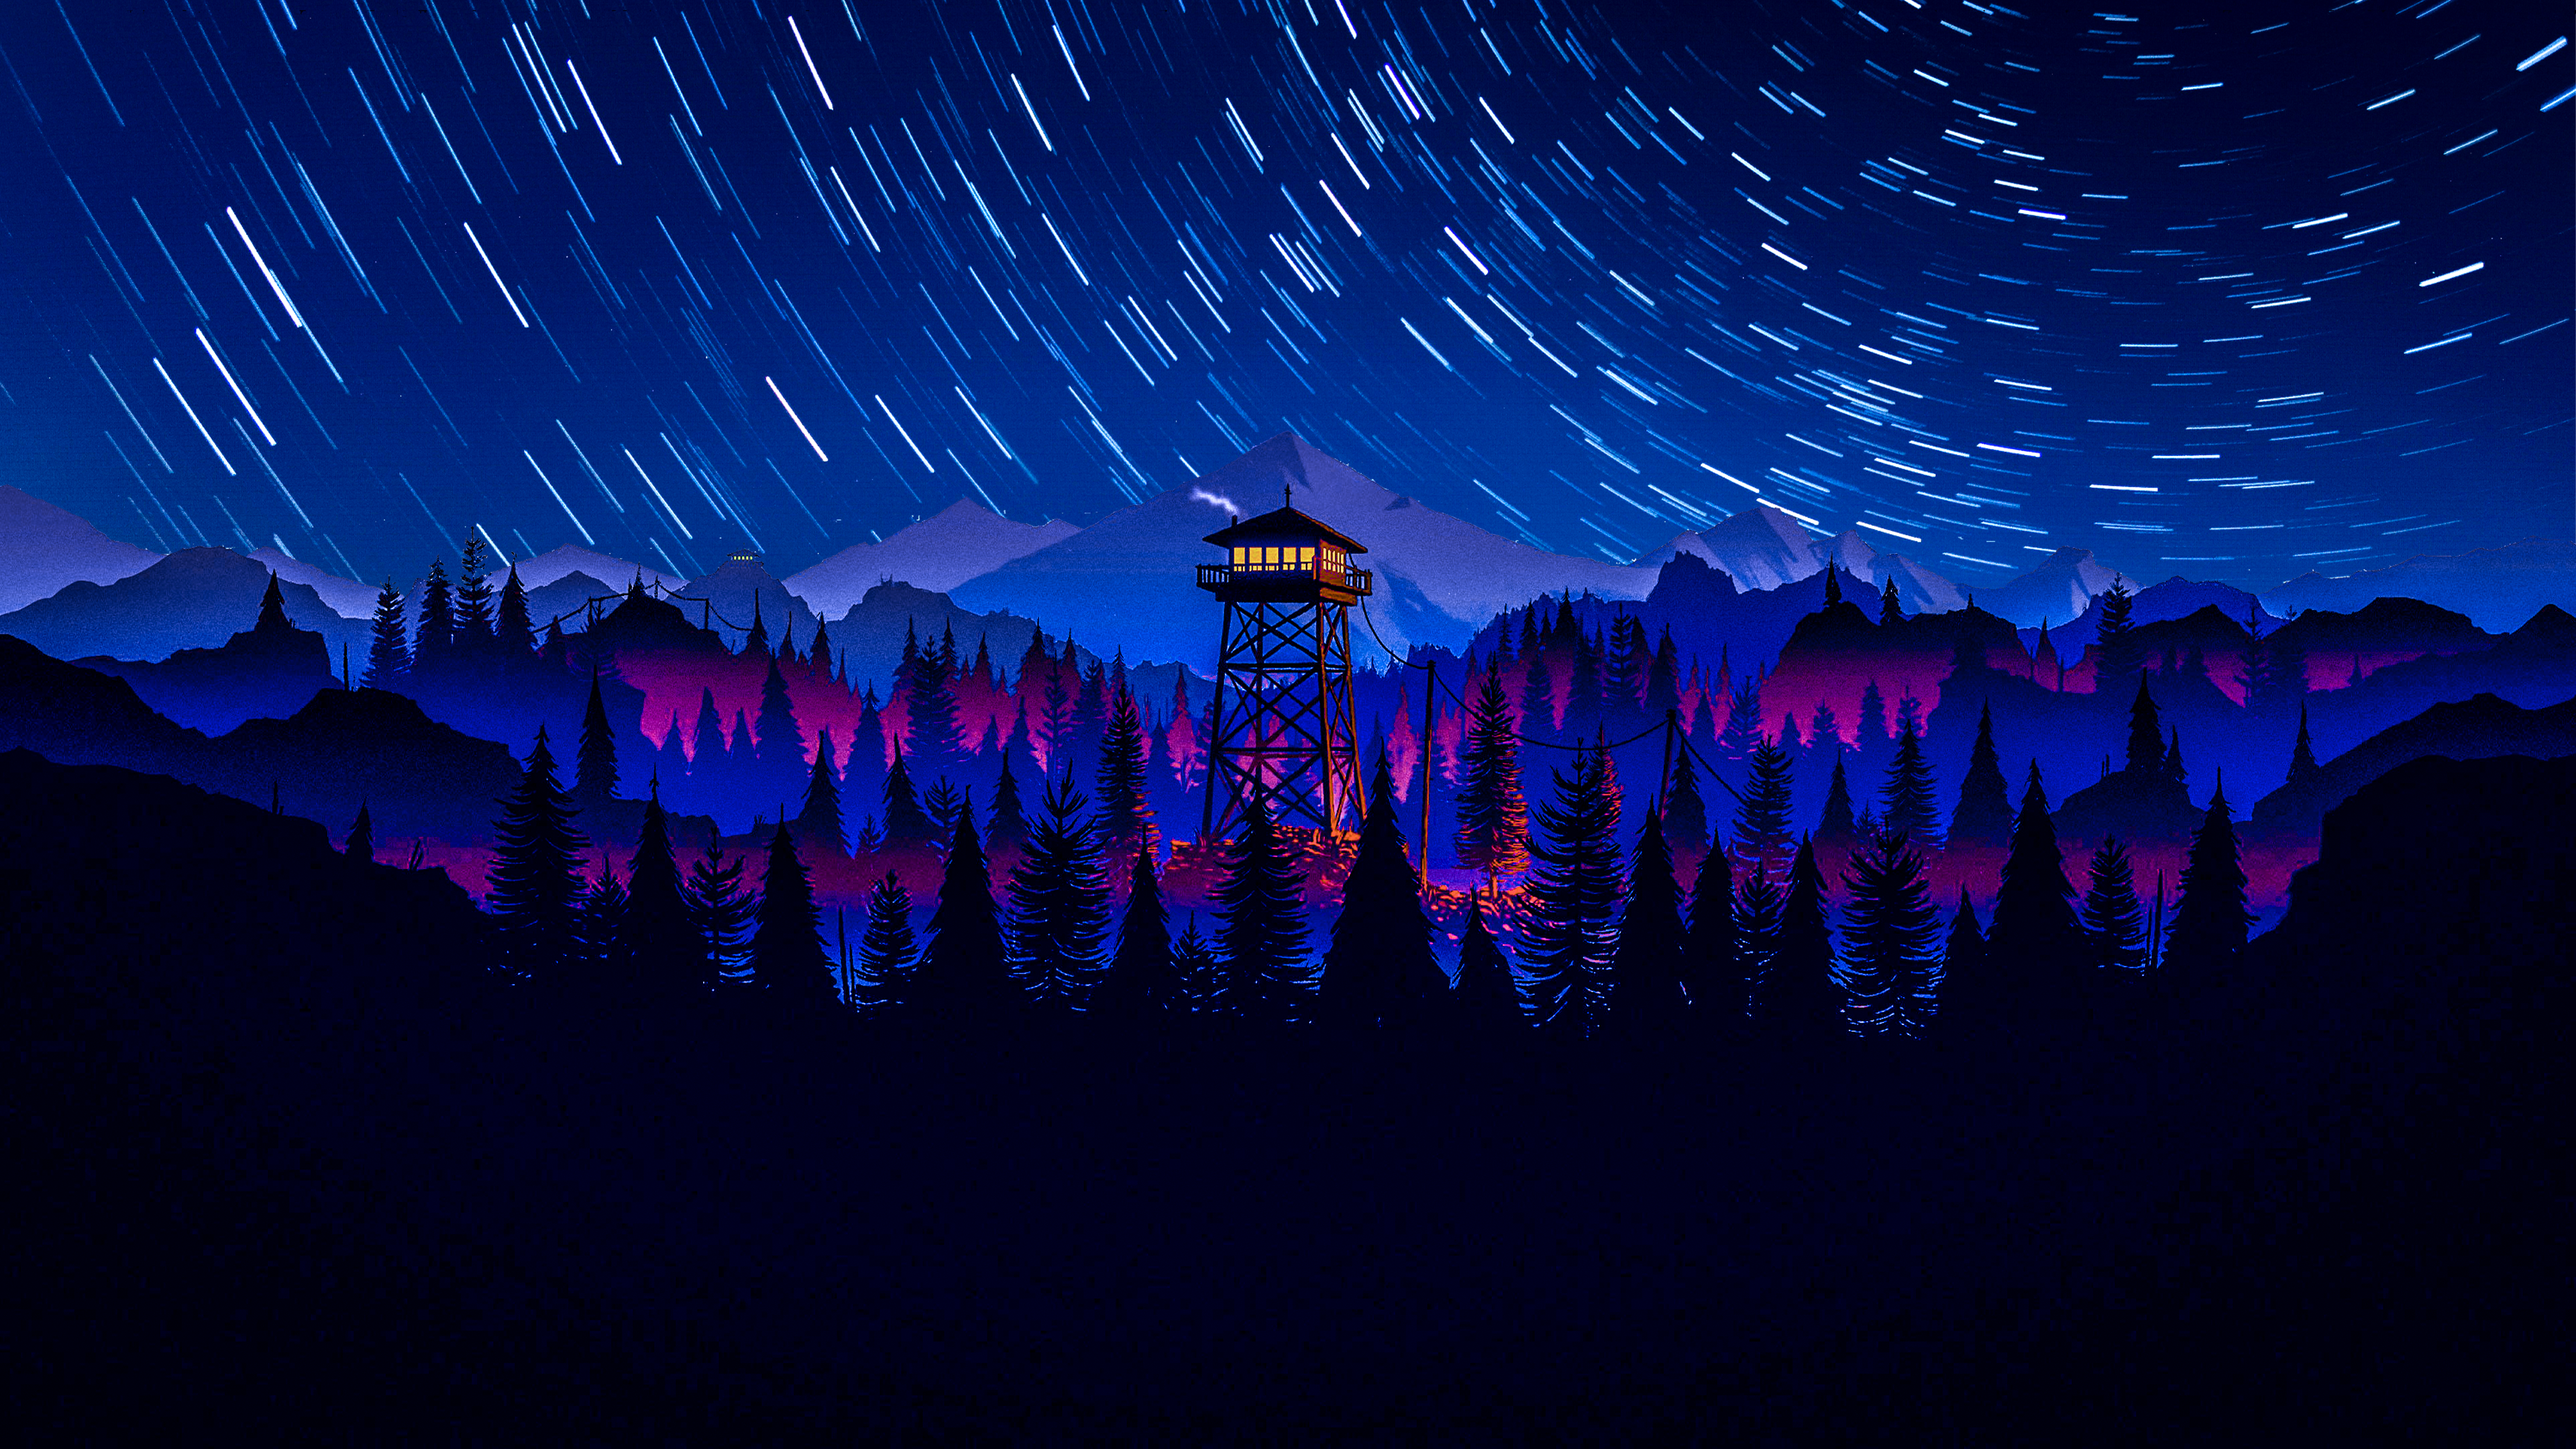
\includegraphics[width=0.75\textwidth]{pictures/KMzdj.png}
    \caption{Firewatch Wallpaper}
    \label{fig:landscape}
\end{figure}


\subsection{Bramka logiczna XOR:}
Tabela~\ref{tab:xor} Tabela pokazuje działa bramki logicznej XOR
    
\begin{table}[htbp]
    \centering
    \begin{tabular}{|c|c|c|}
        \hline \textbf{X} &  \textbf{Y} & \textbf{Z}\\ \hline
        0 & 0 & 0\\ \hline
        1 & 0 & 1\\ \hline
        0 & 1 & 1\\ \hline
        1 & 1 & 0\\ \hline
    \end{tabular}
    \caption{XOR}
    \label{tab:xor}
\end{table}
\subsection{Listy}


\subsubsection{Lista numerowana}
\begin{enumerate}
  \item Element pierwszy
  \item Element drugi
  \item Element trzeci
\end{enumerate}

\subsubsection{Lista nienumerowana}
\begin{itemize}
  \item Element pierwszy
  \item[\#] Element drugi
  \item[!] Element trzeci
\end{itemize}


\subsection{Tekst:}
\textbf{Lorem ipsum} dolor sit amet, consectetur adipiscing elit, sed do eiusmod tempor incididunt ut labore et dolore magna aliqua. \textbf{Ut enim ad minim} veniam, quis nostrud \textit{exercitation ullamco} laboris nisi ut aliquip ex ea commodo consequat. Duis aute irure dolor in reprehenderit in voluptate velit esse cillum  \underline{dolore eu fugiat nulla pariatur.} Excepteur sint occaecat \textbf{cupidatat non} proident, sunt in culpa qui officia deserunt mollit anim id est laborum.